% Dissertationsvorlage der Medizinischen Fakultät Mannheim der Universität Heidelberg, Erstellt von Yannic Meyer auf der Basis der Arbeiten von Patrick Järgen und Julian Gehweiler
%----------------------------------------------------------------------------
%     Präambel
%----------------------------------------------------------------------------
\documentclass{scrreprt}
\KOMAoptions{fontsize=12pt,DIV=calc} %Für druckreifen, zweiseitigen-Satzspiegel die Option "twoside" bei diesem Befehl einfügen und die beiden Befehle in Zeile 22+23 auskommentieren
\usepackage[utf8]{inputenc} %Zeichenkodierung in UTF8
\usepackage[T1]{fontenc} %westeuropäischer Codierung der Schriftart
\usepackage[onehalfspacing]{setspace} %Stellt den Zeilenabstand ein
\KOMAoptions{DIV=12} %Einstellung des Satzspiegels
\usepackage[ngerman]{babel} %Trennungsregeln und autom. Überschriften in n. dt. RS
\usepackage{lmodern} %Verbesserte Standardschriftart
\usepackage{bibgerm} %Paket für deutsche Literaturverzeichnisse
\usepackage{cite} %Sortierung und Kompression von Ziations-Nummern
\usepackage[nottoc]{tocbibind} %Nummerierter Inhaltsverzeichnis-Eintrag für das Literaturverzeichnis
\usepackage[headsepline]{scrlayer-scrpage}
\automark[section]{chapter} %betitelt rechte und linke Seiten mit der Kapitelüberschrift
	\renewcommand*{\chaptermarkformat}{} %keine Chapternummern in Header
	\renewcommand*{\sectionmarkformat}{} %keine Sectionnummern in Header
%=======================
% die folgenden zwei Befehle auskommentieren, wenn in Zeile 6 die twoside-Option aktiviert wurde
\ihead{\headmark} %Header soll immer links gesetzt werden (i=innen, da einseitig=nur rechte Seiten bedeutet)
\chead{} %center Header leer
% die obigen zwei Befehle auskommentieren, wenn in Zeile 7 die twoside-Option aktiviert wurde
%=======================
\renewcommand*\chapterpagestyle{scrheadings} %alle Chapter verwenden die Kopf- und Fußzeile
\usepackage{float} %Basispaket für Floats
\usepackage[format=plain,labelfont=bf,font=small]{caption} %angepasste Abbildungs- und Tabellen-Beschriftungen (http://www.ctan.org/pkg/caption)
\usepackage{array,booktabs} %verbesserte array und tabular-Umgebung
% eigene Befehle für die Zeilenausrichtung in Tabellen. Siehe http://tex.stackexchange.com/questions/12703/how-to-create-fixed-width-table-columns-with-text-raggedright-centered-raggedlef
	\newcolumntype{L}[1]{>{\raggedright\let\newline\\\arraybackslash\hspace{0pt}}m{#1}}
	\newcolumntype{C}[1]{>{\centering\let\newline\\\arraybackslash\hspace{0pt}}m{#1}}
	\newcolumntype{R}[1]{>{\raggedleft\let\newline\\\arraybackslash\hspace{0pt}}m{#1}}
\usepackage{multirow} %erlaubt in einer Tabelle das Setzen von Text über mehrere Tabellen-Zeilen
\usepackage{graphicx} %Ermöglicht Einbindung von Grafiken
\usepackage[space]{grffile} %Erlaubt, mit graphix Dateinamen mit Leerzeichen einzubinden
\usepackage{amsmath} %Bessere Mathematikbereiche
\usepackage[all]{nowidow} %Vermeidet Hurensöhne und Schusterjungen
\usepackage{pdfpages} %pdf-Dateien einbinden
\usepackage{lscape,pdflscape} %Querformat-Darstellung einzelner Seiten
\usepackage{acronym} % Abkürzungen werden beim ersten mal ausgeschrieben, danach abgekürzt
\usepackage{textcomp} % U.a. für Trademark Zeichen (\textsuperscript{TM} or \texttrademark)
\usepackage{todonotes} %erlaubt das einfügen von \todo{To-Dos}

%--------Hilfreiche, aber für das Template nicht zwingend notwendige Pakete. Zur Aktivierung einfach einkommentieren
% \usepackage{textgreek} %Erlaubt Druck von aufrechten griechischen Buchstaben im Text
% \usepackage{siunitx} %Ermöglicht erzeugung komplexerer Maßeinheiten
% \usepackage{varwidth} %Erlaubt erstellen von Minipages mit variabler Breite
%-------------------------------------------------------

%--------Für URL-Breaks in der Bibliographie 
% (siehe https://norwied.wordpress.com/2012/07/10/how-to-break-long-urls-in-bibtex/)
\usepackage{url} %ermöglicht das einbinden klickbarer URLs
\def\UrlBreaks{\do\/\do-\do_\do.\do?}
\usepackage[breaklinks,hidelinks]{hyperref}
%-------------------------------------------------------


%////////////////////////
%     Eigene Befehle -> Hier sind als Beispiele einige eigene LaTeX-Befehle definiert
\clearpage
\newcommand\worry[1]{\textcolor{red}{\textbf{#1}}}
\newcommand{\registered}{\textsuperscript{\textregistered}}
%////////////////////////


%----------------------------------------------------------------------------
%     Deckblatt + 2. Seite
%----------------------------------------------------------------------------

% Info: Das Deckblatt wird in diesem Template mittels der Datei Deckblatt.tex separat generiert und das PDF dann hier eingebunden. 

\begin{document}
\pagenumbering{gobble}

\includepdf[pages={1}]{Deckblatt.pdf} %damit das Deckblatt im oneside Modus eingebunden wird
	\thispagestyle{empty}
	\vspace*{\fill}
	\begin{center}
	Dekan: Prof. Dr. Dekan\\
	Referent: PD. Dr. med. Referent
         \end{center}
%--------------------------------------------------------------------------------------------------
%     Beginn des Dokuments
%--------------------------------------------------------------------------------------------------

%--------------------------------------------------------------------------------------------------
%     Literatur- und Abkürzungsverzeichnis
%--------------------------------------------------------------------------------------------------
\tableofcontents
\thispagestyle{empty}

\cleardoubleoddpage% Damit wir nach dem Umschlag wieder garantiert auf einer rechten Seite sind!
\pagestyle{scrheadings}
\pagenumbering{arabic}

\markboth{\MakeMarkcase{Abkürzungsverzeichnis}}{\MakeMarkcase{Abkürzungsverzeichnis}}

\chapter*{Abkürzungsverzeichnis} 
\addcontentsline{toc}{chapter}{Abkürzungsverzeichnis} \label{sec:abk_Verz}
\begin{acronym}[ABCDE] %längstes Akronym, wird als Mindestabstand verwendet
	\acro{BSP}{Beispiel}
	\acro{MedMa}{Medizin Mannheim}
\end{acronym}

%--------------------------------------------------------------------------------------------------
%     Einleitung
%--------------------------------------------------------------------------------------------------
\chapter{Einleitung}
\section{Diese Vorlage}
Dies Vorlage für eine Dissertation an der Medzinischen Fakultät Mannheim der Universität wurde von Yannic Meyer auf der Basis der Vorarbeit von Patrick Järgen und Julian Gehweiler erstellt und Form und Aufbau sollen noch von der Promotionskommission abgesegnet werden. 

Für die Abfassung der Dissertation sind die entsprechenden Hinweise und Richtlinien der Fakultät zu beachten. In den folgenden Abschnitten finden Sie einige knappe Hinweise zu LaTeX selbst und zur Verwendung dieser Vorlage. 

\paragraph{Einseitiges und Zweiseitiges Layout}
Standardmäßig ist diese Vorlage so eingestellt, dass der Satzspiegel auf der Seite horizontal zentriert wird, da dies für die Betrachtung des generierten PDFs am PC deutlich angenehmer ist. Für einen zweiseitigen Satz, bei dem der Satzspiegel an der Innenfalz einen engeren Abstand hat als beispielsweise zum Rand nach außen kann in der Präambel in Zeile 6 die Option \verb|twoside| eingefügt und Zeile 22 und 23 mit \verb|%| auskommentiert werden. 

\section{Hinweise zu \LaTeX}
\par{\LaTeX} ist eine Textsatzsprache, die schönen Textsatz ermöglicht, sich sehr gut für die Erstellung von Formeln eignet und die Anfertigung von Verzeichnissen (Inhalt, Abbildungen, Tabellen etc.) und Verweisen vereinfacht. Tabellenerstellung oder die Veränderung des verwendeten Templates ist sind dafür aufwändiger als z.B. in MS Word. 

In dieser Dissertationsvorlage der \textit{Medizinischen Fakultät Mannheim} finden Sie in den folgenden Abschnitten einige Beispiele zu Verwendung des Templates. Als Einstieg in LaTeX  ist  \textit{LaTeX - Eine Einführung und ein bisschen mehr} der \textit{Fernuni Hagen} geeignet, um die zu Grunde liegenden Prinzipien zu erlernen \cite{LaTeX_Guide_1}. Es steht auch ein erweiterter Guide (\textit{LaTeX - Fortgeschrittene Anwendungen oder neues von den Hobbits}) zur Verfügung \cite{LaTeX_Guide_2}. Für nahezu alle weiteren Probleme hilft in der Regel eine kurze Recherche bei einer Suchmaschine der Wahl weiter - meist wird man auf \url{https://tex.stackexchange.com} fündig. 

\section{Abbildungen und Tabellen}

Abbildungen und Tabellen können als sog. \textit{floats} gesetzt werden und tauchen daher nicht, wie man es evtl. aus Word kennt, \textit{zwingend} an der Stelle im Text, wo sie definiert sind, sondern LaTeX versucht, sie nach einem gewissen Regelwerk optimal unterzubringen. Die Definition \verb|htpb| gibt an, dass der \textit{float} \verb|here|, auf der oberen (\verb|top|) oder unteren (\verb|bottom|) Hälfte einer Seite oder auf einer eigenen Seite (\verb|page|) gesetzt wird. Mit der Option \verb|H| kann die Positionierung an Ort und Stelle erzwungen werden. Die Optimierung der Abbildungsplatzierung sollte möglichst erst gegen Ende der Fertigstellung der Dissertation erfolgen, um erneute Verschiebungen durch Textveränderungen zu vermeiden. 

Eine Anleitung zur Erstellung übersichtlicher und visuell ansprechender Tabellen findet sich in der Dokumentation des Paketes \verb|booktabs| auf \url{http://ftp.math.purdue.edu/mirrors/ctan.org/macros/latex/contrib/booktabs-de/booktabs-de.pdf}. Zur Erstellung von Abbildungen gibt es von Rougier et al. ein paar hilfreiche Hinweise auf \url{http://dx.plos.org/10.1371/journal.pcbi.1003833} \cite{Rougier2014}. 
\vspace*{0.6cm}

\begin{figure}[htpb] %Beispielabbildung
	{\centering
		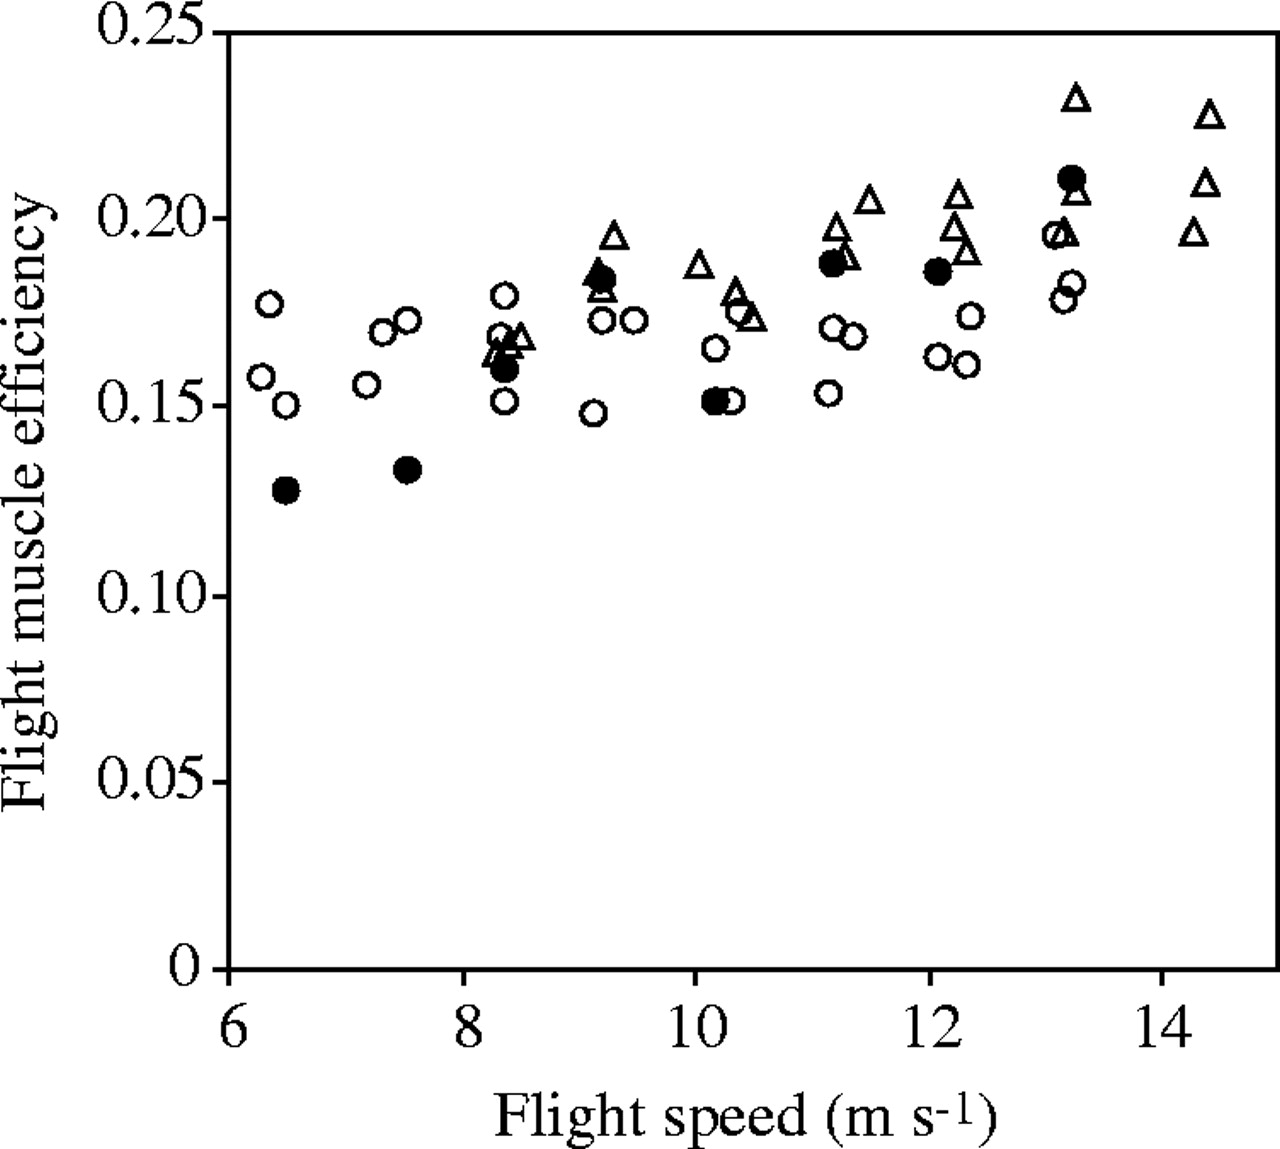
\includegraphics[height=6cm]{abbildungen/Starling_Mechpower.jpg} 
		\caption[Mechanische Leistung eines Staren im Windtunnel]{
			\textbf{Mechanische Leistung eines Staren im Windtunnel.} 
			Flug-Muskel-Effizienz von zwei Staren während eines Windtunnel-Fluges. Pmech gibt die mechanische Leistung an ($\bullet$ Vogel 15, Pmech anhand des Vortex-Ring-Modells geschätzt; $\circ$ Vogel 15, Pmech anhand des Linien-Auftriebs Modells geschätzt; $\triangle$ Vogel 19, Pmech anhand des Linien-Auftriebs-Modells geschätzt). (Abbildung von Ward et al. übernommen  \cite{Ward2001}).
			}
		\label{fig:beispielabbildung}
	}
\end{figure}


\begin{table}[htpb] %Beispieltabelle
	\begin{center}
		\renewcommand{\arraystretch}{1.0} %Hier lässt sich der Zeilenabstand vergrößern/verkleinern
		\small
		\begin{tabular}{C{2cm}C{2cm}C{2.2cm}C{2.2cm}C{2cm}C{2cm}}
			\toprule
			\textbf{Flight Speed} [m/s] & \textbf{Frequency} [Hz] &\textbf{ Wingbeat amplitude} [degrees] & \textbf{Down-stroke ratio} & \textbf{Stroke plane angle} [degrees] & \textbf{Wingspan} [m] \\
			\midrule
			6,5 & 10,3 & 57,5 & 0,546 & 55,6 & 0,354 \\
			7,6 & 10,2 & 43,5 & 0,480 & 65,7 & 0,399 \\
			8,4 & 10,5 & 53,9 & 0,475 & 64,3 & 0,348 \\
			9,2 & 10,7 & 62,0 & 0,465 & 72,8 & 0,348 \\
			10,2 & 10,6 & 50,3 & 0,494 & 71,1 & 0,377 \\
			11,2 & 11,4 & 65,6 & 0,482 & 78,3 & 0,353 \\
			12,1 & 11,3 & 64,1 & 0,478 & 83,5 & 0,358 \\
			13,3 & 11,0 & 63,0 & 0,484 & 80,8 & 0,380 \\
			\bottomrule
		\end{tabular}
		\caption[Flügelschlag-Kinematik eine Staren]{
			\textbf{Flügelschlag-Kinematik von Vogel 15.}
			Die Messungen erfolgten mittels Hochgeschwindigkeits-Videoaufzeichnungen während eines Windtunnelfluges durch Vogel 15 mit Atemmaske. (Tabelle von Ward et al. übernommen  \cite{Ward2001}).
			}
		\label{tab:beispieltabelle}
	\end{center}
\end{table}

\section{Querverweise und Abkürzungsverzeichnis} \label{sec:verweise}
Zur Verwendung von \textbf{Querverweisen} kann an jeder Stelle im Text ein \verb|\label{label}| platziert werden und seine Nummer kann mit \verb|\ref{label}| und seine Seitenzahl mit \\ \verb|\pageref{label}| abgerufen werden. Befindet sich das Label einfach im Text wird die Nummer des Abschnittes zugewiesen, befindet sich das Label in einer Abbildung oder Tabelle wird die entsprechende Nummer der fortlaufenden Abbildungs- und Tabellen-Nummerierung ausgegeben (So trägt dieser Abschnitt die Nummer \ref{sec:verweise} und befindet sich auf S. \pageref{sec:verweise}). 

Ein \textbf{Abkürzungsverzeichnis} kann wie auf S. \pageref{sec:abk_Verz} definiert und auf die Abkürzungen mittels \verb|\ac{Abkürzung}| zugegriffen werden. In der aktuellen Konfiguration wird bei der ersten Nennung die Lang- und Kurzebezeichnung (\ac{BSP}) ausgegeben, bei weiteren dann nur die Kurzbezeichnung (\ac{BSP}). 


\section{Bibliographie}

Zur Erstellung einer Bibliographie mit \verb|BibTex| und \verb|BibLaTeX| zwei verschiedene Schnittstellen zur Verfügung. Mit z.B. EndNote kann automatisiert die eine BibTex-Datei für die Literaturliste generiert werden, in der jedem Eintrag der Datenbank ein Zitations-Schlüssel zugewiesen wird (eine Anleitung findet sich z.B. hier: \url{http://libguides.mit.edu/c.php?g=176170&p=1158648#3}). Der Zitations-Schlüssel kann mit \verb|\cite{schlüssel}| abgerufen werden und LaTeX übernimmt, wie man es z.B. vom Endnote-Plugin für Word kennt, die Nummerierung und Erstellung des Literaturverzeichnisses. Die Referenz-Datei für das Literaturverzeichnis ist hier an der entsprechenden Stelle im Code mit \\ \verb|\bibliography{BibTex/library}| eingebunden, der Befehl  \verb|\bibliographystyle{ieeetr}| generiert dann das Literaturverzeichnis. 

\section{Was noch zu tun ist}
Mit dem \verb|todonotes|-Paket kann eine To-Do-Liste geführt werden. Die Notizen können einfach mit \verb|\todo{das ist noch zu erledigen!}| eingefügt werden. Weitere Informationen finden sich in der Dokumentation des Paketes: \url{https://www.ctan.org/pkg/todonotes}.

%--------------------------------------------------------------------------------------------------
%     Material Methoden
%--------------------------------------------------------------------------------------------------

\chapter{Material und Methoden}\label{sec:materialmethoden}

\section{Sektion}\label{sec:Sektion1}
Lorem ipsum dolor sit amet, consetetur sadipscing elitr, sed diam nonumy eirmod tempor invidunt ut labore et dolore magna aliquyam erat, sed diam voluptua. At vero eos et accusam et justo duo dolores et ea rebum. Stet clita kasd gubergren, no sea takimata sanctus est Lorem ipsum dolor sit amet. Lorem ipsum dolor sit amet, consetetur sadipscing elitr, sed diam nonumy eirmod tempor invidunt ut labore et dolore magna aliquyam erat, sed diam voluptua. At vero eos et accusam et justo duo dolores et ea rebum. Stet clita kasd gubergren, no sea takimata sanctus est Lorem ipsum dolor sit amet.
\section{Subsektion}
Lorem ipsum dolor sit amet, consetetur sadipscing elitr, sed diam nonumy eirmod tempor invidunt ut labore et dolore magna aliquyam erat, sed diam voluptua. At vero eos et accusam et justo duo dolores et ea rebum. Stet clita kasd gubergren, no sea takimata sanctus est Lorem ipsum dolor sit amet. Lorem ipsum dolor sit amet, consetetur sadipscing elitr, sed diam nonumy eirmod tempor invidunt ut labore et dolore magna aliquyam erat, sed diam voluptua. At vero eos et accusam et justo duo dolores et ea rebum. Stet clita kasd gubergren, no sea takimata sanctus est Lorem ipsum dolor sit amet.
\subsubsection{Sub-Subsektion} 
Lorem ipsum dolor sit amet, consetetur sadipscing elitr, sed diam nonumy eirmod tempor invidunt ut labore et dolore magna aliquyam erat, sed diam voluptua. At vero eos et accusam et justo duo dolores et ea rebum. Stet clita kasd gubergren, no sea takimata sanctus est Lorem ipsum dolor sit amet. Lorem ipsum dolor sit amet, consetetur sadipscing elitr, sed diam nonumy eirmod tempor invidunt ut labore et dolore magna aliquyam erat, sed diam voluptua. At vero eos et accusam et justo duo dolores et ea rebum. Stet clita kasd gubergren, no sea takimata sanctus est Lorem ipsum dolor sit amet.
\paragraph{Absatzüberschrift}
Lorem ipsum dolor sit amet, consetetur sadipscing elitr, sed diam nonumy eirmod tempor invidunt ut labore et dolore magna aliquyam erat, sed diam voluptua. At vero eos et accusam et justo duo dolores et ea rebum. Stet clita kasd gubergren, no sea takimata sanctus est Lorem ipsum dolor sit amet. Lorem ipsum dolor sit amet, consetetur sadipscing elitr, sed diam nonumy eirmod tempor invidunt ut labore et dolore magna aliquyam erat, sed diam voluptua. At vero eos et accusam et justo duo dolores et ea rebum. Stet clita kasd gubergren, no sea takimata sanctus est Lorem ipsum dolor sit amet.


%--------------------------------------------------------------------------------------------------
%     Ergebnisse
%--------------------------------------------------------------------------------------------------
% Ziel: Ca. 15 Seiten
\chapter{Ergebnisse}

\section{Sektion}
\section{Subsektion}

%--------------------------------------------------------------------------------------------------
%     Diskussion
%--------------------------------------------------------------------------------------------------
	
\chapter{Diskussion}

\section{Sektion}
\section{Subsektion}

%--------------------------------------------------------------------------------------------------
%     Zusammenfassung
%--------------------------------------------------------------------------------------------------

\chapter{Zusammenfassung}


%--------------------------------------------------------------------------------------------------
%     Tabellen- und Abbildungsverzeichnisse
%--------------------------------------------------------------------------------------------------

\listoffigures

\listoftables


%--------------------------------------------------------------------------------------------------
%     Literaturverzeichnis
%--------------------------------------------------------------------------------------------------
\bibliography{BibTex/library} 
\bibliographystyle{ieeetr}


%--------------------------------------------------------------------------------------------------
%     Tabellarischer Anhang
%--------------------------------------------------------------------------------------------------
\chapter*{Anhang}
\addcontentsline{toc}{chapter}{Anhang}  



%--------------------------------------------------------------------------------------------------
%     Lebenslauf
%--------------------------------------------------------------------------------------------------

\chapter*{Lebenslauf}
\addcontentsline{toc}{chapter}{Lebenslauf}  

\begin{tabular}{p{4cm}l}
	\multicolumn{2}{l}{{\large \scshape{Personalien}}} \\[0,6em]
	
	Name und Vorname:	& Marina Musterfrau \\[0,5em]
	
	Geburtsdatum: 		& 01.01.1970 \\[0,5em]
	
	Geburtsort: 		& Mannheim \\[0,5em]
	
	Familienstand: 		& Ledig\\[0,5em]
	
	Vater: 				& Maximilian Musterfrau \\[0,5em]
	
	Mutter: 			& Mörte Musterfrau \\[0,5em]
	& \\[0,5em]
	\multicolumn{2}{l}{{\Large \scshape{Schulischer Werdegang}}} \\[0,6em]
	
	1976 - 1980: 	& Grundschule Mannheim\\[0,5em]

	1980 - 1990: 	& Gymnasium Mannheim\\[0,5em]

	Abitur: 			& 09.06.1990 \\[0,5em]
	&\\[0,5em]
		\multicolumn{2}{l}{{\Large \scshape{Universitärer Werdegang}}} \\[0,6em]
	WS2010/2011			& Beginn des Studiums der Humanmedizin an der \\
						& Universität Heidelberg, Medizinische Fakultät Mannheim\\ [0,5em]
						
	<Datum> 		& 1. Abschnitt der Ärztlichen Prüfung\\
	<Datum> 		& 2. Abschnitt der Ärztlichen Prüfung
\end{tabular}


%--------------------------------------------------------------------------------------------------
%     Danksagung
%--------------------------------------------------------------------------------------------------

\chapter*{Danksagung}
\addcontentsline{toc}{chapter}{Danksagung}  


\end{document}
%--------------------------------------------------------------------------------------------------
%     Ende des Dokuments
%--------------------------------------------------------------------------------------------------
